\documentclass{standalone}
\usepackage{tikz}
\usepackage{ctex,siunitx}
\setCJKmainfont{Noto Serif CJK SC}
\usepackage{tkz-euclide}
\usepackage{amsmath}
\usetikzlibrary{patterns, calc,3d}
\usetikzlibrary {decorations.pathmorphing,decorations.pathreplacing,decorations.shapes}
\tikzset{label style/.append style={font=\small}}
\begin{document}
\small
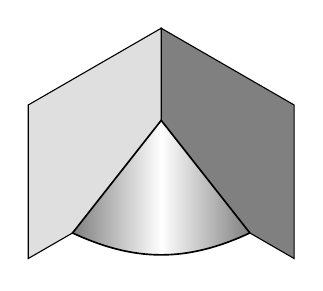
\begin{tikzpicture}[>=latex,scale=1.3,z={(-150:1cm)},x={(-30:1cm)}]
\draw[fill=gray](0,0,0)--(1.5,0,0)--(1.5,1.5,0)--(0,1.5,0)--cycle;
\draw[fill=lightgray!50](0,0,0)--(0,0,1.5)--(0,1.5,1.5)--(0,1.5,0)--cycle;
\draw[left color=gray,right color=gray,middle color=white,semithick](1,0,0)--(0,0.6,0)--(0,0,1)to[bend right=25](1,0,0);
\end{tikzpicture}
\end{document}